\documentclass[a4paper,12pt,oneside,onecolumn,openany,final]{memoir}

%Preamble
%-----------------------------------------------------------------------------------------
\usepackage{thesis_preamble}

\title{Applications of Galois Theory}
\author{Sandesh Thakuri}
\date{March 2024}

%------------------------------------------------------------------------------------------

\begin{document}

\frontmatter
% --------------------------------------------------------------------------------------------

\begin{center}
  {\LARGE
    {\bfseries {\MakeTextUppercase {\thetitle}}}} \\

  \vspace{1.5cm}

\begin{figure}[h]
	\centering
	\includegraphics[height=5cm,width=5cm]{pictures/tulogo.png}
\end{figure}

\vspace{2cm}

	THESIS SUBMITTED TO\\ THE
	 CENTRAL DEPARTMENT OF MATHEMATICS\\
	INSTITUTE OF SCIENCE AND TECHNOLOGY\\
	TRIBHUVAN UNIVERSITY \\
	KATHMANDU, NEPAL\\

\vspace{1.5cm}

	BY\\
	{\bfseries SANDESH THAKURI}

\vspace{1.5cm}

SUBMITTED FOR THE\\
PARTIAL FULFILLMENT OF THE REQUIREMENT FOR\\
THE MASTER IN SCIENCE/ARTS (M.SC./M.A.)  DEGREE\\
IN MATHEMATICS\\

\vspace{1.5cm}

MARCH, 2024

\end{center}

%\underbrace{}
\thispagestyle{empty}

\clearpage
\begin{center}
	\includegraphics[width=0.15\textwidth]{tulogo.png}\\[1.5cm]
\end{center}

\begin{center}
	{\color{white}a}\\
\vspace{15.0cm}
\textcopyright~2024\\
Sandesh Thakuri\\
All Rights Reserved
\end{center}
\thispagestyle{empty}
\clearpage

\addcontentsline{toc}{chapter}{\bfseries DEDICATION}
\begin{center}
	\includegraphics[width=0.15\textwidth]{pictures/tulogo.png}
\end{center}
\begin {center}
\vspace{1.5cm}

{\Large{\bfseries {DEDICATION}}}\\[2cm]

To\\[0.5cm]
My Parents\\
{\bfseries {\color{blue} Sharada Thakuri and Prem Bdr. Thakuri.}}\\[8mm]
%Along with\\
%My ......\\
%{\bf{\color{blue}Name}}\\[8mm]
\end {center}

\clearpage
\addcontentsline{toc}{chapter}{\bfseries STUDENT DECLARATION}
 %\vspace{-1cm}


\begin{center}
  \includegraphics[width=0.15\textwidth]{pictures/tulogo.png}\\[1.5cm]

    {\Large{\bfseries{STUDENT'S DECLARATION}}}\\[.5cm]

  \end{center}


This thesis entitled ``\textbf{\thetitle}", which has been submitted to the Central Department of Mathematics, Institute of Science and Technology (IOST), Tribhuvan University, Nepal for the partial fulfillment of the Master in Science/Arts (M.Sc./M.A.) Degree  in Mathematics, is a genuine work that I carried out under my supervisor {\color{red} Assoc. Prof. Tulasi Prasad Nepal} and that no sources other than those listed in the Bibliography have been used in this work. Moreover, this work has not been published or submitted elsewhere for the requirement of any degree programme.
\\[1.5cm]
-----------------------\\
\theauthor\\
Batch: $2077$ \\
TU Registration Number: 5-2-37-1874-2016\\ \\
Date: March, 2024

\clearpage
\addcontentsline{toc}{chapter}{\bfseries RECOMMENDATION}

\vspace{-1cm}
\begin{center}
	\includegraphics[width=0.15\textwidth]{pictures/tulogo.png}\\[1.5cm]
	{\Large{\bfseries{RECOMMENDATION}}}\\[.5cm]
      \end{center}

This is to recommend that Mr. \textbf{\theauthor} has prepared this thesis entitled ``\textbf{\thetitle}" for the partial fulfillment of the Master in Science/Arts (M.Sc./M.A.) in Mathematics under my supervision. To my knowledge, this work has not been submitted for any other degree.
He has fulfilled all the requirements laid down by the Central Department of Mathematics, Institute of Science and Technology (IOST), Tribhuvan University (TU), Kirtipur for the submission of the thesis for the partial fulfillment of M.Sc./M.A. Degree in Mathematics.\\

\vspace{1.5cm}
\noindent
..............................\\
Mr. Tulasi Prasad Nepal\\
\textbf {Supervisor}\\
%Central Department of Mathematics\\ Tribhuvan University, Kirtipur\\
Associate Professor\\ \\
Date: March, 2024

\clearpage
 \addcontentsline{toc}{chapter}{\bfseries LETTER OF APPROVAL}

 \begin{center}
 	\includegraphics[width=0.15\textwidth]{pictures/tulogo.png}\\[1.5cm]
 {\Large{\bfseries{LETTER OF APPROVAL}}}\\[.5cm]
\end{center}

\noindent
We certify that the Research Evaluation Committee of the Central Department of Mathematics, Tribhuvan University, Kirtipur approved this research work entitled ``\textbf{\thetitle}" carried out by Mr. \textbf{\theauthor} in the scope and generality as a thesis in the partial fulfillment for the requirement of the M.Sc./M.A. degree in Mathematics.
\\[3.5cm]
\begin{minipage}{0.45\textwidth}
                ......................................\\[2mm]
                (\textbf{External Examiner})\\
                Dr. Santosh Ghimire\\
                Pulchowk Campus,\\
                Institute of Engineering,\\
                Tribhuvan University,\\
                Kathmandu, Nepal.\\
		Date: \thedate
\end{minipage} \hspace{3mm}
%
\begin{minipage}{0.55\textwidth}
                ......................................\\
                (\textbf{Supervisor}) \\
		Assoc. Prof. Tulasi Prasad Nepal \\
		Central Department of Mathematics,\\
                Institute of Science \& Technology,\\
                Tribhuvan University,\\
                Kirtipur, Kathmandu, Nepal.\\[0.1cm]
		Date: \thedate

\end{minipage}\\[3cm]

\begin{center}
  ........................................\\
  	(\textbf{Head of Department})\\
        Prof. Dr. Chet Raj Bhatta\\
        Central Department of Mathematics\\
	 Institute of Science \& Technology\\
	 Tribhuvan University, Kathmandu,
	 Kirtipur,Nepal.\\
	Date: \thedate
\end{center}

\addcontentsline{toc}{chapter}{\bfseries ACKNOWLEDGMENTS}

\begin{center}
{\Large{\bfseries ACKNOWLEDGMENTS}}
\end{center}

\vspace{1cm}
First of all I would like to thank my \textbf{supervisor} Mr. Tulasi Prasad Nepal(Associate Professor of Central Department of Mathematics).\\

I am thankful to former HOD of the department Prof. Dr. Tanka Nath Dhamala for his valuable support and time. Then I am thankful to Santosh Gyanwali sir for providing me the necessary articles. Then I am thankful to my friends and family.
\\[5cm]

\begin{minipage}{1\textwidth}
	\begin{flushright}
		%
		....................................\\
		{\bfseries Sandesh Thakuri}\\
		Date: \thedate
		%
	\end{flushright}
\end{minipage}

\clearpage
\addcontentsline{toc}{chapter}{\bfseries ABSTRACT}
\begin{center}
{\Large{\bfseries ABSTRACT}}
\end{center}
\vspace{0.7cm}

In this thesis entitled \textcolor{blue}{\thetitle}, a brief but complete theory of Galois is developed in the first part. Then its applications are explored in the second and third part. The second part deals with the applications in Algebra where as the third part deals with the applications in computer science. The application in algebra is the famous classic problem of non-existence of a ``formula'' for a polynomial of degree greater than four. The application in computer science is the application of ``Galois field'' in Coding theory and Cryptography.\\

The new research in this thesis is the computation of Galois group of a fifth degree and of a seventh degree polynomial and extension of Galois group from single variable polynomial to multi-variable polynomial.

\clearpage
\addcontentsline{toc}{chapter}{\bfseries {Symbol Conventions Used}}

\hspace{-7mm}
  {\LARGE {\bfseries {Symbol Conventions}}}

  \vspace{7mm}

Through out the thesis following Symbol Convention has been used.\\[4mm]

\begin{itemize}
\item \textbf{K} \hspace{5mm} a field.
\item \textbf{F} \hspace{5mm} an extension field of the field \textbf{K}
\end{itemize}

\section*{Some Standard Symbols}
\begin{enumerate}
\item \(\mathbb{Z}\) \hspace{5mm} set of integers.
\item \(\mathbb{Q}\) \hspace{5mm} set of rationals.
\item \(\mathbb{R}\) \hspace{5mm} set of reals.
\item \(\mathbb{C}\) \hspace{5mm} set of complex numbers.
\item \(\mathbb{Z}_n\) \hspace{5mm} ring of set of integers modulo \(n\).
\item \(\mathbb{Z}_p\) \hspace{5mm} finite prime field.
  \item AES \hspace{5mm} American Encryption Standard.
\end{enumerate}
\clearpage


%\maxtocdepth{subsection} % put 3 levels into the ToC
\tableofcontents  %table of contents
\listoffigures*
\listoftables*

\mainmatter
% ---------------------------------------------------------------------------------------------
\part{Galois Theory}
\addtocontents{toc}{\protect\mbox{}\protect\hrulefill\par}

\chapter{Field Extension}
\section{Structure of a Field Extension}
Let \(F=K(u)\) be a field extension of the field \(K\). Then \(F\) is a vector space over \(K\) generated by \(u\).\\
We have \(u^n \in F\) for all \(n \in \mathbb{Z}\) because F is a field. As \(F\) is a vector space over \(K\); \(F\) consists of all linear combinations of \(u^n \)'s, and the quotients of these linear combinations. A such linear combinations is: \(a_nu^n+a_{n-1}u^{n-1}+...+a_1u+a_0\) which is  given by the polynomial \(f(u)\), where \(f(x)=a_nx^n+a_{n-1}x^{n-1}+...+a_1x+a_0\).\\

So the structure of the extension field \(F=K(u)\) is:\\
\(F= \{\frac{f(u)}{g(u)} \;| \; f,g \in K[x],g(u) \neq 0\}\).\\

\begin{theorem}[Existence of an Extension field]
If K is a field and \(f \in K[x]\) is a polynomial of degree \(n\),then there exists a simple extension field \(F=K(u)\) of K such that \(u\in F\) is a root of \(f\).
\end{theorem}

\subsection{Algebraic and Transcendental element}
\begin{theorem}
Let \(F\) be an extension field of a field \(F\).\\
A map \(\phi:K[X] \rightarrow K[u]\) where \(u \in F\) defined by \(\phi (f(x))=f(u)\)\\
i.e, \(\phi (a_0+a_1x+...+a_nx^n)= a_0+a_1u+...+a_nu^n\) is a ring homomorphism.
\end{theorem}

Thus \( K[x]\) and \(K[u]\) are homomorphic.
  \begin{enumerate}
  \item If \(u\) is transcendental over \(K\) then \(K[u]\) is not a field and \(K[x] \cong K[u]\).
  \item If \(u\) is algebraic over \(K\) then, \(K[x] \ncong K[u]\) because \(Ker\phi\) is non trival and we have,
    \begin{enumerate}
    \item[i)] \(K(u) \cong K[u]\);
    \item[ii)] \(K(u) \cong K[x]/(f)\), where \(f \in K[x]\) is an 'irreducible monic polynomial of degree \(n \geq 1\);
    \item[iii)] \([K(u):K]=n\) and \(\{1_k,u,u^2,...,u^{n-1}\}\) is a basis of the vector space \(K(u) over K\).
    \end{enumerate}
  \end{enumerate}

\begin{theorem}[Isomorphism of Extension fields]
 Let K be a field.\\
 Then 'u' and 'v' are  roots of the same irreducible polynomial \(f \in K[x]\) if and only if there is an isomorphism of fields \(K[u] \cong K[v]\) which sends u onto v and is the identity on \(K\).
\end{theorem}

\section{Galois Group}
Let \(F\) be a field. The set \(AutF\) of all field-automorphisms \(F \rightarrow F \) forms a group under the function composition.\\ \\
Let \(E\) and \(F\) be the extension fields of a field \(K\).\\
If a non-zero field-homomorphism \(\sigma : E \rightarrow F\) is a K-module homomorphism then\\
\(\sigma(k)=\sigma(k1_E)=k\sigma(1_E)=k1_F=k\).\hspace{7mm}
i.e, \(\sigma\) fixes \(K\) element-wise.\\
Conversely, if a field homomorphism \(\sigma : E \rightarrow F\) fixes K element-wise, then \(\sigma\) is a non-zero and for any \(u \in E\), we have, \(\sigma(ku)=\sigma(k)\sigma(u)=k\sigma(u)\)
i.e \(\sigma\) is a K-module homomorphism.\\
\begin{definition}
  A field-automorphism \(\sigma \in Aut F\) which is also K-homomorphism is called K-automorphism. In other words, a field-automorphism \(\sigma \in Aut F\) that fixes K element-wise is called K-automorphism.
\end{definition}

\begin{definition}
  The group of all K-automorphisms of \(F\) is called the Galois group of \(F\) over \(K\) and it is denoted by \(Aut_K^F\).
\end{definition}

\section{Galois extension}
Let \(E\) be an intermediate field and \(H\) be a subgroup of \(Aut_K^F\), then:
\begin{enumerate}
\item[i)] \(H' = \{v \in F \; | \: \sigma(v)=v,\) for all \(\sigma \in H \}\) is an intermediate field of the extension field \(F\) of \(K\);
\item[ii)] \(E' = \{\sigma \in Aut_K^F \; | \; \sigma(u)=u,\) for all \(u \in E\}=Aut_E^F\) is a subgroup of \(Aut_K^F\).
\end{enumerate}

The field \(H'\) is called the fixed field of the subgroup H in F.

\subsection{Fixed Field}
We have,\\
\(H' \rightarrow\) fixed field and \(E' \rightarrow\) \(Aut_E^F\).\hspace{5mm} Let \(Aut_K^F = G\) then the field fixed by it is \(G'\). It is not necessary that the field fixed by \(G\) is \(K\) i.e, \(G'=K\).
\begin{example}
For \(f(x)=x^3-2 \in Q[x]\). Let \(u \in F\) such that \(f(u)=0\) and let \(F=Q[u]\).Then
\(G=Aut_Q^{Q(u)}={1}\) so, \hspace{5mm}\(G'=F \neq K\).\\
\end{example}

\begin{definition}
  Let \(F\) be an extension field of \(K\) such that the fixed field of the Galois group \(Aut_K^F\) is \(K\) itself. Then \(F\) is said to be a Galois extension of \(K\) or Galois over \( K\).
\end{definition}

\section{Fundamental Theorem of Galois Theory}
\begin{theorem}
If \(F\) is a finite dimensional Galois extension of \(K\), then there is a one-to-one correspondence between the set of all intermediate fields of \(F\) over \(K\) and the set of subgroups of the Galois group \(Aut_K^F\) such that:
\begin{enumerate}
\item[i)] the relative dimension of two intermediate fields is equal to the relative index of the corresponding subgroups. In particular \(Aut_K^F\) has order \([F:K]\);
  \item[ii)] \(F\) is Galois over every intermediate field \(E\), but \(E\) is Galois over \(K\) if and only if the corresponding subgroup \(E'= Aut_E^F\) is normal in \(G=Aut_K^F\).In this case \(G/E'\) is isomorphic to the Galois group \(Aut_K^E\) of \(E\) over \(K\).
  \end{enumerate}
\end{theorem}
We already have a correspondence between the intermediate fields and the subgroup of Galois group.\\
That is to each intermediate field \(E\), there is a subgroup \(Aut_E^F\) and to each subgroup \(H\) there is a fixed field \(H'\). But this correspondence is one-to-one if and only if for each intermediate field \(E\), it satisfies \(E''=E\) and for each subgroup \(H\), it satisfies \(H''=H\).

  \subsection{Closed Field and Subgroup}
  We have,
  \begin{enumerate}
  \item[i)] \(F'=1\) and \(K'=G\);
  \item[ii)] \(1'=F\);
    \end{enumerate}

    If \(F\) is Galois over \(K\) then by definition, \(G'=K\). Since \(K'=G\) we have \(K=K''\) if and only if \(F\) is Galois over \(K\).\\

\begin{definition}
  Let \(X\) be an intermediate field or subgroup of the Galois group. \(X\) will be called \textbf{closed} provided \(X=X''\).\\
\end{definition}

\begin{lemma}. If \(F\) is an extension field of \(K\), then there is one-to-one correspondence between the closed intermediate fields of the extension and the closed subgroups of the Galois group, given by \(E \rightarrow E' =  Aut_E^F\).\\
\end{lemma}

\begin{lemma}. Let \(F\) be an extension field of \(K\), \(L\) and \(M\) intermediate fields with \(L \subset M\), and \(H\), \(J\) subgroups of Galois group \(Aut_K^F\) with \(H<J\).
    \begin{enumerate}
    \item[i)] If \(L\) is closed and \([M:L]\) finite, then \(M\) is closed and \([L':M']=[M:L]\);
    \item[ii)] if \(H\) is closed and \([J:H]\) finite, then \(J\) is closed and \([H':J']=[J:H]\);
      \item[iii)] if \(F\) is a finite dimensional Galois extension of \(K\), then all intermediate fields and all subgroups of the Galois group are closed and \(Aut_K^F\) has order \([F:K]\).
\end{enumerate}
\end{lemma}


\subsection{Stable Intermediate}
\begin{lemma}
Let \(F\) be an extension field of K.
      \begin{enumerate}
      \item[i)] If E is a stable intermediate field of the extension, then \(E'=Aut_E^F\) is a normal subgroup of the Galois group \(Aut_K^F\);
        \item[ii)] if \(H\) is a normal subgroup of \(Aut_K^F\), then the fixed field \(H'\) of \(H\) is a stable intermediate field of the extension.
        \end{enumerate}
        \end{lemma}

        \subsection{Proof of the Fundamental Theorem}
        \begin{proof}
From the above section there is one-to-one correspondence between closed intermediate fields of the extension and closed subgroups of the Galois group. But in this case all intermediate fields and all subgroups are closed. Thus follows statement(i) of the theorem.\\

        \(F\) is Galois over \(E\) since \(E\) is closed. \(E\) is finite dimensional over \(K\) since \(F\) is and hence algebraic over \(K\). Consequently, if \(E\) is Galois over \(K\), then \(E\) is stable.
        \(E'=Aut_E^F\) is normal in \(Aut_K^F\). Conversely if \(E'\) is normal in \(Aut_K^F\), then \(E''\) is stable intermediate field. But \(E=E''\) since all intermediate fields are closed and hence \(E\) is Galois over \(K\).\\

       Suppose \(E\) is an intermediate field that is Galois over \(K\). Since \(E\) and \(E'\) are closed and \(G'=K\)(F is Galois over K), we have \(|G/E'|=[G:E']=[E''=G']=[E:K]\). So, \(G/E'=Aut_K^F/Aut_E^F\) is isomorphic to a subgroup of \(Aut_K^F\). But by first part of the theorem, \(|Aut_K^E|=[E:F]\)(since E is Galois over K). This implies \(G/E'=Aut_K^E\).
        \end{proof}


%%% Local Variables:
%%% mode: latex
%%% TeX-master: "n"
%%% End:


\chapter{Galois Correspondence}
\section{Galois Group}
Let \(F\) be a field. ``The set \(AutF\) of all field-automorphisms \(F \rightarrow F \) forms a group under the function composition'' \cite{hunger}.\\[3mm]
\noindent
Let \(E\) and \(F\) be the extension fields of a field \(K\).\\
If a non-zero field-homomorphism \(\sigma : E \rightarrow F\) is a K-module homomorphism then\\
\(\sigma(k)=\sigma(k1_E)=k\sigma(1_E)=k1_F=k\).\hspace{7mm}
i.e, \(\sigma\) fixes \(K\) element-wise.\\
Conversely, if a field homomorphism \(\sigma : E \rightarrow F\) fixes K element-wise, then \(\sigma\) is a non-zero and for any \(u \in E\), we have, \(\sigma(ku)=\sigma(k)\sigma(u)=k\sigma(u)\)
i.e \(\sigma\) is a K-module homomorphism \cite{hunger}.
\begin{definition} \cite{hunger}
  A field-automorphism \(\sigma \in Aut F\) which is also K-homomorphism is called K-automorphism. In other words, a field-automorphism \(\sigma \in Aut F\) that fixes K element-wise is called K-automorphism.
\end{definition}

\begin{definition} \cite{hunger}
  ``The group of all K-automorphisms of \(F\) is called the Galois group of \(F\) over \(K\) and it is denoted by \(Aut_K^F\).''
\end{definition}

\section{Galois extension}
Let \(E\) be an intermediate field and \(H\) be a subgroup of \(Aut_K^F\), then:
\begin{enumerate}
\item[i)] ``\(H' = \{v \in F \; | \: \sigma(v)=v,\) for all \(\sigma \in H \}\)'' \cite{hunger} is an intermediate field of the extension field \(F\) of \(K\);
\item[ii)] ``\(E' = \{\sigma \in Aut_K^F \; | \; \sigma(u)=u,\) for all \(u \in E\}=Aut_E^F\)'' \cite{hunger} is a subgroup of \(Aut_K^F\).
\end{enumerate}

The field \(H'\) is called the fixed field of the subgroup H in F \cite{hunger}.

\subsection{Fixed Field}
We have,\\
\(H' \rightarrow\) fixed field and \(E' \rightarrow\) \(Aut_E^F\).\hspace{5mm} Let \(Aut_K^F = G\) then the field fixed by it is \(G'\). It is not necessary that the field fixed by \(G\) is \(K\) i.e, \(G'=K\).
\vspace{3mm}
\begin{example}
  For \(f(x)=x^3-2 \in Q[x]\). Let \(u \in F\) such that \(f(u)=0\) and let \(F=Q[u]\).Then
  \(G=Aut_Q^{Q(u)}={1}\) so, \hspace{5mm}\(G'=F \neq K\).
\end{example}

\vspace{3mm}
\begin{definition} \cite{hunger}
``Let \(F\) be an extension field of \(K\) such that the fixed field of the Galois group \(Aut_k^F\) is \(K\) itself. Then \(F\) is said to be a Galois extension of \(K\) or Galois over K.''
\end{definition}

\section{Fundamental Theorem of Galois Theory}
\begin{tcolorbox}
\begin{theorem} \cite{hunger}
  ``If \(F\) is a finite dimensional Galois extension of \(K\), then there is a one-to-one correspondence between the set of all intermediate fields of \(F\) over \(K\) and the set of subgroups of the Galois group \(Aut_K^F\) such that:
  \begin{enumerate}
  \item[i)] the relative dimension of two intermediate fields is equal to the relative index of the corresponding subgroups. In particular \(Aut_K^F\) has order \([F:K]\);
  \item[ii)] \(F\) is Galois over every intermediate field \(E\), but \(E\) is Galois over \(K\) if and only if the corresponding subgroup \(E'= Aut_E^F\) is normal in \(G=Aut_K^F\).In this case \(G/E'\) is isomorphic to the Galois group \(Aut_K^E\) of \(E\) over \(K\).''
  \end{enumerate}
\end{theorem}
\end{tcolorbox}

\vspace{2mm}
We already have a correspondence between the intermediate fields and the subgroup of Galois group.\\
That is to each intermediate field \(E\), there is a subgroup \(Aut_E^F\) and to each subgroup \(H\) there is a fixed field \(H'\). But this correspondence is one-to-one if and only if for each intermediate field \(E\), it satisfies \(E''=E\) and for each subgroup \(H\), it satisfies \(H''=H\).

\subsection{Closed Field and Subgroup}
\begin{definition} \cite{hunger}
  ``Let \(X\) be an intermediate field or subgroup of the Galois group. \(X\) will be called \textbf{closed} provided \(X=X''\).''
\end{definition}
\clearpage

\begin{lemma} \cite{hunger}
\begin{enumerate}
\item[i)] If \(F\) is an extension field of \(K\), then there is one-to-one correspondence between the closed intermediate fields of the extension and the closed subgroups of the Galois group, given by \(E \rightarrow E' =  Aut_E^F\).
\item[ii)] If \(F\) is a finite dimensional Galois extension of \(K\), then all intermediate fields and all subgroups of the Galois group are closed and \(Aut_K^F\) has order \([F:K]\).
  \end{enumerate}
\end{lemma}
\vspace{3mm}

\subsection{Stable Intermediate}
\begin{definition} \cite{hunger}
  An intermediate field \(E\) of \(F\) over \(K\) is said to be stable intermediate if \(\sigma(E) \subseteq E\) for every \(\sigma \in Aut_K^F\) .
\end{definition}

\begin{lemma} \cite{hunger}
  \begin{enumerate}
  \item[i)] If E is a stable intermediate field of the extension, then \(E'=Aut_E^F\) is a normal subgroup of the Galois group \(Aut_K^F\) ;

  \item[ii)] if \(H\) is a normal subgroup of \(Aut_K^F\), then the fixed field \(H'\) of \(H\) is a stable intermediate field of the extension
  \end{enumerate}
\end{lemma}
\vspace{3mm}

\subsection{Proof of the Fundamental Theorem}
\begin{proof}
From lemma 1 above, one-to-one correspondence between the intermediate fields and the subgroups follows \cite{hunger}. And from lemma 2 the next two statements of the theorem follows \cite{hunger}.
\end{proof}
\vspace{3mm}

\section{Application}
The fundamental theorem links Field theory to Group theory. This allows us to use the tools of Group theory to solve the problems involving field theory. Solving a polynomial equation is a problem of field theory. We can use insights of Group theory to solve this problem of field theory which is discussed in some detail in next part of this thesis \cite{hunger}.
\clearpage

\section{Illustration of The Fundamental Theorem}
\begin{minipage}{0.68\textwidth}
  Let \(F\) be an Galois extension of a field \(K\). Let the towers of the intermediate fields of \(F\) over \(K\) be as follows:
  \[
    K \subset E \subset F
  \]
\noindent
  Let \(G\) be the Galois group of \(F\) over \(K\). Then its subsets are
  \[
    \{e\} \subset H \subset G
  \]
  Then the one-to-one correspondence is as shown:
\end{minipage}\hspace{2mm}
\begin{minipage}{0.3\textwidth}

  \begin{tcolorbox}[colback=gray!20, colframe=blue!20, title={\footnotesize \textcolor{black}{Galois-correspondence}}, width=5cm]
    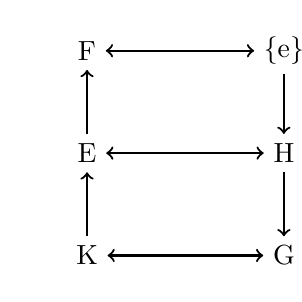
\begin{tikzpicture}
      \hspace{5mm}
      \node (f) {F};
      \node[below of=f, yshift=-3mm] (e) {E};
      \node[below of=e, yshift=-3mm] (k) {K};

      \draw[<-,thick] (f)--(e);
      \draw[<-,thick] (e)--(k);

      \node[right of=f, xshift=15mm] (i) {\{e\}};
      \node[below of=i, yshift=-3mm] (h) {H};
      \node[below of=h, yshift=-3mm] (g) {G};

      \draw[->, thick] (i)--(h);
      \draw[->, thick] (h)--(g);

      \draw[<->, thick] (f)--(i);
      \draw[<->, thick] (e)--(h);
      \draw[<->, thick] (k)--(g);
    \end{tikzpicture}
  \end{tcolorbox}
\end{minipage}

\vspace{5mm}
\begin{remark}
  The intermediate fields are getting larger as we go from top to bottom  as the fields are getting extended. But the subgroups are getting smaller.
\end{remark}

\vspace{7mm}
\section{Insights to the Fundamental Theorem}

\subsection{Nature of a Number}
The nature of a number depends upon the underlying field. As a field-automorphism of  \(\mathbb{Q}(\sqrt{2})\) that fixes \(\mathbb{Q}\) is \(\mathbb{Q}(-\sqrt{2})\) i.e \(\sqrt{2} \longmapsto -\sqrt{2}\). So,  any polynomial equation over \(\mathbb{Q}\) satisfied by the number \(\sqrt{2}\) is also satisfied by the number \(-\sqrt{2}\). You can fluidly pass between these two numbers and the equation with a rational coefficient will not know. \textit{Hence the two numbers \(\sqrt{2}\) and \(-\sqrt{2}\) are algebraically same over \(\mathbb{Q}\).}\\

But the map \(\sqrt{2} \longmapsto -\sqrt{2}\) is not an automorphism of the field \(\mathbb{Q}(\sqrt{2})\) fixing itself, i.e fixing \(\mathbb{Q}(\sqrt{2})\). The only automorphism of \(\mathbb{Q}(\sqrt{2})\) is the identity map. So, you cannot pass \(\sqrt{2}\) for \(-\sqrt{2}\) for every equation with coefficients in \(\mathbb{Q}(\sqrt{2})\). \textit{Hence the two numbers \(\sqrt{2}\) and \(-\sqrt{2}\) are not algebraically same over \(\mathbb{Q}(\sqrt{2})\).}
\vspace{7mm}

\begin{figure}[h]
  \centering
 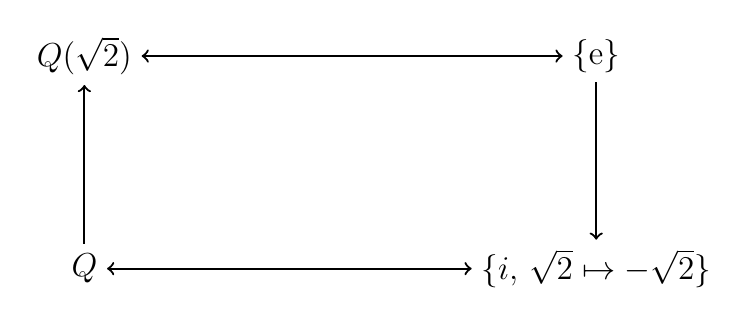
\begin{tikzpicture}
      \node (f) {\large \(\mathbb{Q}(\sqrt{2})\)};
      \node[below of=f, yshift=-17mm] (e) {\large \(\mathbb{Q}\)};


      \draw[<-,thick] (f)--(e);

      \node[right of=f, xshift=55mm] (i) {\large \{e\}};
      \node[below of=i, yshift=-17mm] (h) {\large \{\(i\), \(\sqrt{2} \mapsto -\sqrt{2}\)\}};


      \draw[->, thick] (i)--(h);


      \draw[<->, thick] (f)--(i);
      \draw[<->, thick] (e)--(h);
    \end{tikzpicture}
    \end{figure}
\clearpage

\subsection{Structure of a Field}
The structure of a field as an extension field over some field is mirrored in the structure of the ``group'' of  permutations of its elements that keeps the base field fixed. But these permutations are the symmetries of the field. \textit{So, the structure of field extension is equals to its own symmetry.}\\

The structure of a field is a \textbf{complicated} thing; specially if it is infinite. But the structure of a group is rather simple; especially if it is finite. So the Galois theory has fairly simplified the complicated thing in a very insightful and beautiful way.\\

Also Galois theory gives a new sights of study of fields which is ``study of fields via study of its automorphisms'' which are permutations of the field. That is\\[5mm]

\begin{figure}[h]
  \centering
  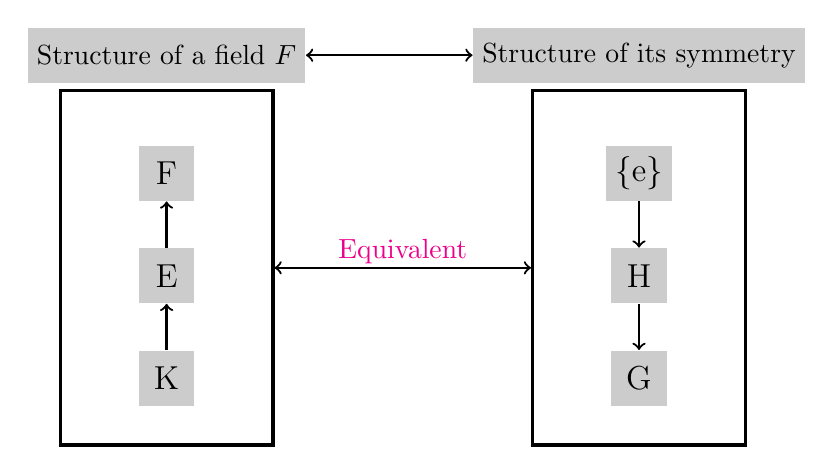
\begin{tikzpicture}

    \node[rectangle, very thick, draw,
    minimum height=4.5cm,
    minimum width=2.7cm] (rec) at (0,0) {};

    \node[rectangle, very thick, draw,
    minimum height=4.5cm,
    minimum width=2.7cm] (rec2) at (6,0) {};


    \node[minimum width=7mm,
      minimum height=7mm,
      fill=gray!40,
      ] (ss) at (0,2.7) {Structure of a field \(F\)};

      \node[minimum width=7mm,
      minimum height=7mm,
      fill=gray!40,
      ] (ss2) at (6,2.7) {Structure of its symmetry};

      \draw[<->, thick] (ss)--(ss2);
       \draw[<->, thick] (rec)--(rec2);

      \node[minimum width=7mm,
      minimum height=7mm,
      fill=gray!40] (f) at (0,1.2) {\large F};

      \node[minimum width=7mm,
      minimum height=7mm,
      fill=gray!40,
      below of=f, yshift=-3mm] (e) {\large E};

      \node[right of=e,
      xshift=20mm, yshift=3mm] (txt) {\textcolor{magenta}{Equivalent}};

      \node[minimum width=7mm,
      minimum height=7mm,
      fill=gray!40,
      below of=e, yshift=-3mm] (k) {\large K};

      \draw[<-,thick] (f)--(e);
      \draw[<-,thick] (e)--(k);

      \node[right of=f,
      xshift=5cm,
      minimum width=7mm,
      minimum height=7mm,
      fill=gray!40,
      ] (i) {\large \{e\}};

      \node[minimum width=7mm,
      minimum height=7mm,
      fill=gray!40,
      below of=i, yshift=-3mm] (h) {\large H};

      \node[
      minimum width=7mm,
      minimum height=7mm,
      fill=gray!40,
      below of=h, yshift=-3mm] (g) {\large G};

      \draw[->, thick] (i)--(h);
      \draw[->, thick] (h)--(g);
    \end{tikzpicture}
    \caption{\footnotesize Equivalency}
\end{figure}


\chapter{Structure of Galois Extension}
\section{Galois Group}
Let \(F\) be a field. The set \(Aut F\) of all field-automorphisms \(F \rightarrow F \) forms a group under the function composition.\\ \\
Let \(E\) and \(F\) be extension fields of a field \(K\).\\
If nonzero field-homomorphism \(\sigma : E \rightarrow F\) is a K-module homomorphism then\\
\(\sigma(k)=\sigma(k1_E)=k\sigma(1_E)=k1_F=k\).\hspace{7mm}
i.e, \(\sigma\) fixes \(K\) elementwise.\\ \\
Conversely, if field homomorphism \(\sigma : E \rightarrow F\) fixes K elementwise, then \(\sigma\) is a nonzero and for any \(u \in E\),\(\sigma(ku)=\sigma(k)\sigma(u)=k\sigma(u)\)
i.e \(\sigma\) is a K-module homomorphism.\\ \\
A field-automorphism \(\sigma \in Aut F\) which is also K-homomorphism is called K-automorphism. In other words, a field-automorphism \(\sigma \in Aut F\) that fixes K elementwise is called K-automorphism.\\ \\
The group of all K-automorphisms of \(F\) is called the Galois group of \(F\) over \(K\) and is denoted by \(Aut_K^F\).

\section{Galois extension}
Let \(E\) be an intermediate field and \(H\) be a subgroup of \(Aut_K^F\), then:
\begin{enumerate}
\item[i)] \(H' = \{v \in F | \sigma(v)=v, for all \sigma \in H \}\) is an intermediate field of the extension field \(F\) of \(K\).
\item[ii)] \(E' = \{\sigma \in Aut_K^F | \sigma(u)=u, for all u \in E\}=Aut_E^F\) is a subgroup of \(Aut_K^F\).
\end{enumerate}

The field \(H'\) is called the fixed field of subgroup H in F.

\subsection{Fixed Field}
We have,\\
\(H' \rightarrow fixed field \) \hspace{5mm} \(E' \rightarrow Aut_E^F\)\\
Let \(Aut_K^F = G\) then the field fixed by it is \(G'\).\\
It is not necessary that the field fixed by \(G\) is \(K\) i.e, \(G'=K\).\\

\textbf{Example}\\
For \(f(x)=x^3-2 \in Q[x]\). Let \(u \in F\) such that \(f(u)=0\) and \(F=Q[u]\).Then
\(G=Aut_Q^{Q(u)}={1}\) so, \(G'=F \neq K\).\\[2mm]

\textbf{Galois extension}\\
Let \(F\) be an extension field of \(K\) such that the fixed field of the Galois group \(Aut_K^F\) is \(K\) itself. Then \(F\) is said to be a Galois extension of \(K\) or to be Galois over \( K\).

\section{Fundamental Theorem of Galois Theory}

If \(F\) is a finite dimensional Galois extension of \(K\), then there is a one-to-one correspondence between the set of all intermediate fields of the extension and the set of subgroups of the Galois group \(Aut_K^F\) such that:
\begin{enumerate}
\item[i)] the relative dimension of two intermediate fields is equal to the relative index of the corresponding subgroups; in particular \(Aut_K^F\) has order \([F:K]\);
  \item[ii)] \(F\) is Galois over every intermediate field \(E\), but \(E\) is Galois over \(K\) if and only if the corresponding subgroup \(E'= Aut_E^F\) is normal in \(G=Aut_K^F\);in this case \(G/E'\) is isomorphic to the Galois group \(Aut_K^E\) of \(E\) over \(K\).
  \end{enumerate}

  We already have a correspondence between the intermediate fields and the subgroup of Galois group given by the fixed fields and the corresponding subgroups of the intermediate field \(E\), \(Aut_E^F\).
  i.e, to each intermediate field \(E\), there is a subgroup \(Aut_E^F\) and to each subgroup \(H\) there is a fixed field \(H'\).\\[2mm]
  But this correspondence is one-to-one if and only if \(E''=E\) and so on.

  \subsection{Closed Field and Subgroup}
  We have,
  \begin{enumerate}
  \item[i)] \(F'=1\) and \(K'=G\);
  \item[ii)] \(1'=F\);
    \end{enumerate}

    If \(F\) is Galois over \(K\) then by definition, \(G'=K\). Since \(K'=G\) we have \(K=K''\) if and only if \(F\) is Galois over \(K\).\\

    Let \(X\) be an intermediate field or subgroup of the Galois group. \(X\) will be called \textbf{closed} provided \(X=X''\).\\[3mm]

    \textbf{Theorem}. If \(F\) is an extension field of \(K\), then there is one-to-one correspondence between the closed intermediate fields of the extension and the closed subgroups of the Galois group, given by \(E \rightarrow E' =  Aut_E^F\).\\[3mm]

    \textbf{Lemma}. Let \(F\) be an extension field of \(K\), \(L\) and \(M\) intermediate fields with \(L \subset M\), and \(H\), \(J\) subgroups of Galois group \(Aut_K^F\) with \(H<J\).
    \begin{enumerate}
    \item[i)] If \(L\) is closed and \([M:L]\) finite, then \(M\) is closed and \([L':M']=[M:L]\);
    \item[ii)] if \(H\) is closed and \([J:H]\) finite, then \(J\) is closed and \([H':J']=[J:H]\);
      \item[iii)] if \(F\) is a finite dimensional Galois extension of \(K\), then all intermediate fields and all subgroups of the Galois group are closed and \(Aut_K^F\) has order \([F:K]\).
      \end{enumerate}

      \subsection{Stable Intermediate}
      \textbf{Lemma}. Let \(F\) be an extension field of K.
      \begin{enumerate}
      \item[i)] If E is a stable intermediate field of the extension, then \(E'=Aut_E^F\) is a normal subgroup of the Galois group \(Aut_K^F\);
        \item[ii)] if \(H\) is a normal subgroup of \(Aut_K^F\), then the fixed field \(H'\) of \(H\) is a stable intermediate field of the extension.
        \end{enumerate}

        \subsection{Proof of the Fundamental Theorem}
        From the above section there is one-to-one correspondence between closed intermediate fields of the extension and closed subgroups of the Galois group. But in this case all intermediate fields and all subgroups are closed. Thus follows Statement(i) of the theorem.\\[2mm]

        \(F\) is Galois over \(E\) since \(E\) is closed. \(E\) is finite dimensional over \(K\) since \(F\) is and hence algebraic over \(K\). Consequently, if \(E\) is Galois over \(K\), then \(E\) is stable.
        \(E'=Aut_E^F\) is normal in \(Aut_K^F\). Conversely if \(E'\) is normal in \(Aut_K^F\), then \(E''\) is stable intermediate field. But \(E=E''\) since all intermediate fields are closed and hence \(E\) is Galois over \(K\).\\[2mm]

        Suppose \(E\) is an intermediate field that is Galois over \(K\). Since \(E\) and \(E'\) are closed and \(G'=K\)(F is Galois over K), we have \(|G/E'|=[G:E']=[E''=G']=[E:K]\). So, \(G/E'=Aut_K^F/Aut_E^F\) is isomorphic to a subgroup of \(Aut_K^F\). But by first part of the theorem, \(|Aut_K^E|=[E:F]\)(since E is Galois over K). This implies \(G/E'=Aut_K^E\).



%%% Local Variables:
%%% mode: latex
%%% TeX-master: "n"
%%% End:


\part{Applications in Algebra}
\addtocontents{toc}{\protect\mbox{}\protect\hrulefill\par}

\chapter{Galois Group of a Polynomial}
\begin{definition}
  The Galois group of a polynomial \(f \in K[x]\) is the group \(Aut_K^F\), where \(F\) is a splitting field of \(f\) over \(K\).
  \end{definition}

  \begin{theorem}
  Let \(G\) be a Galois group of a polynomial \(f \in K[x]\).
\begin{enumerate}
\item[i)] \(G\) is isomorphic to a subgroup of some symmetric group \(S_n\)..
  \item[ii)] If \(f\) is separable of degree \(n\), the \(n\) divides \(|G|\) and \(G\) isomorphic to a transitive subgroup of \(S_n\).
  \end{enumerate}
\end{theorem}
Because the Galois group \(Aut_K^F\) is a group of automorphisms of F which is given by the permutations of the roots.
So, the Galois group of a polynomial is identified with the subgroup of \(S_n\).\\

\begin{corollary}
\begin{enumerate}
\item[i)] If the degree of \(f\) is \(2\) then its Galois group \(G \cong {\mathbb{Z}}_2\).
  \item[ii)] If the degree of \(f\) is \(3\) then its Galois group \(G\) is either \(S_3\) or \(A_3\).
  \end{enumerate}
\end{corollary}


\section{Galois Group of Cubic polynomials}
\begin{definition}
  Let \(K\) be a field with \(char K \neq 2\) and \(f \in K[x]\) a polynomial of degree \(n\) with \(n\) distinct roots \(u_1,u_2,...,u_n\) in some splitting field \(F\) of \(f\) over \(K\). Let \(\Delta = \prod\limits_{i<j}(u_i-u_j) = (u_1-u_2)(u_1-u_3)...(u_{n-1}-u_n) \in F\).\\
  The discriminant of \(f\) is the element \(D= {\Delta}^2\).
\end{definition}

\begin{theorem}
\begin{enumerate}
\item[i)] The discriminant \({\Delta}^2\) of \(f\) actually lies in \(K\).
  \item[ii)] For each \(\sigma \in Aut_K^F < S_n, \sigma\) is an even[resp. odd] if and only if \(\sigma(\Delta) = \Delta\)[resp. \(\sigma(\Delta) = - \Delta\)].
  \end{enumerate}
\end{theorem}
Since \({\Delta}^2 \in K\) and \(\Delta \in F\), and \(K(Delta)\) is a stable intermediate; in the Galois correspondence the subfield \(K(\Delta)\) corresponds to the subgroup \(G \cap A_n\). In particular, \(G\) consists of even permutations if and only if \(\Delta \in K\).

\begin{corollary}
  If \(f\) is a separable polynomial of degree \(3\), then the Galois group of \(f\) is \(A_3\) if and only if the discriminant of \(f\) is the square of an element of \(K\).
\end{corollary}

\begin{theorem}
  Let \(K\) be a field of \(char K \neq 2,3 \). If \(f(x)=x^3+bx^2+cx+d \in K[x]\) has three distinct roots in some splitting field, then the polynomial \(g(x)=f(x-b/3) \in K[x]\) has the form \(x^3+p^2+q\) and the discriminant of \(f\) is \(-4p^3-27q^2\) ~\cite{hunger}.
\end{theorem}

\section{Galois Group of Quartic polynomials}
\begin{definition}[Resolvant Cubic of a Quartic]
Let \(K, f, F, u_i, V,\) and \(G=Aut_K^F<S_4\) be as in the preceding paragraph and \(\alpha=u_1u_2+u_3u_4,\) \(\beta=u_1u_3+u_2u_4,\) \(\gamma=u_1u_4+u_2u_3\).
The polynomial \( (x- \alpha)(x- \beta)(x- \gamma) \) is called the resolvant cubic of \(f\). The resolvant cubic is actually a polynomial over \(K\).\\
\end{definition}
Now under the Galois correspondence the subfield \(K(\alpha, \beta, \gamma)\) corresponds to the normal subgroup \(V \cap G\) because \(K(\alpha,\beta,\gamma)\) is a splitting field of the resolvant cubic
whose Galois group is a subgroup of \(S_3\) and only normal subgroup of \(N\) of \(S_4\) with \(|N| \leq 6\) is \(V\).\\
Hence \(K(\alpha, \beta, \gamma)\) is Galois over \(K\) and \(Aut_K^{K(\alpha, \beta, \gamma)} = G/(G \cap V\).

\begin{remark} If \(K\) is a field and \(f = x^4+bx^3+cx^2+dx+e \in K[x]\), then the resolvant cubic of \(f\) is the polynomial \(x^3-cx^2+(bd-4e)x-b^2e+4ce-d^2 \in K[x]\).\\ \\
\end{remark}

\begin{theorem}
  Let \(K\) be a field and \(f \in K[x]\) a separable quartic with Galois Group \(G\). Let \(\alpha, \beta, \gamma\) be the roots of the resolvant cubic of \(f\) and let \(m= [K(\alpha, \beta, \gamma) : K]\) then,
\begin{enumerate}
\item[i)] \(m=6 \Longleftrightarrow G=S_4\);
\item[ii)] \(m=3 \Longleftrightarrow G=A_4\);
\item[iii)] \(m=1 \Longleftrightarrow G=V\);
\item[iv)] \(m=2 \Longleftrightarrow G=D_4\) or \(G={\mathbb{Z}}_4\); in this case \(G={\mathbb{Z}}_4\) if \(f\) is irreducible over \(K(\alpha, \beta, \gamma)\) and \(G={\mathbb{Z}}_4\) otherwise.
  \end{enumerate}
\end{theorem}
This is because we have \([K(\alpha,\beta,\gamma):K] = |G/G \cap V|\).

\section{Galois Group of some Polynomials}

\begin{example}
The polynomial is \(f(x)=x^4-2 \in \mathbb{Q}[x]\).\\
This polynomial is irreducible and so separable over \(\mathbb{Q}\). The resolvant cubic is \(x^3+8x = x(x+2i\sqrt{2})(x-2i\sqrt{2})\) and 
\(\mathbb{Q}(\alpha,\beta, \gamma)=\mathbb{Q}(i\sqrt{2})\) has dimension \(2\) over \(mathbb{Q}\).\\
\(x^4-2\) is irreducible over \(\mathbb{Q}(i\sqrt{2})\) because \(\sqrt[\leftroot{-3}\uproot{3}4]{2} \not\in \mathbb{Q}(i\sqrt{2})\).
Therefore the Galois group \(G \cong D_8\).
\end{example}








%%% Local Variables:
%%% mode: latex
%%% TeX-master: "n"
%%% End:


\chapter{The Classic Problem}
\begin{enumerate}
\item Is every polynomial equation solvable by the method of radicals?
\item Equivalently, does there exist an explicit "formula" which gives all solutions of a polynomial equation?
\end{enumerate}

``If the degree of  the polynomial \(f\) is at most four then the answer is \textbf{yes}'' \cite{hunger}.

\section{Formulation of the Classic Problem}
The formula by the method of radicals means the ``formula involving only field operations and the extraction of \(nth\) roots'' \cite{hunger}.
``The existence of a formula means there is a finite sequence of steps, each step being a field operatioin or the extraction of an \(nth\) roots, which yields all solutions of the given polynomial.
Performing a field operatioin leaves the base field unchanged, but the extraction of an \(nth\) root of an element
\(c\) in a field \(K\) amounts to constructing an extenstion field \(K(u)\) with \(u^n \in K\). Thus the existence of a formula for solving \(f(x)=0\) would imply
the existence of a finite tower of fields
\[K=E_0 \subset E_1 \subset ... \subset E_n\]
such that \(E_n\) contains a splitting field of \(f\) over \(K\) and for each \(i \geq 1\), \(E_i=E_{i-1}(u_i)\) with some positive power of \(u_i\) lying in \(E_{i-1}\)'' \cite{hunger}.\\
``Conversely suppose there exists such a tower of fields and that \(E_n\) contains a splitting field of \(f\). Then
\[E_n = K(u_1,u_2,...,u_n)\]
and each solution is of the form \(f(u_1,...,u_n)/g(u_1,...,u_n)\) where \(f,g \in K[x_1,...,x_n]\). \\
Thus each solution is expressible in terms of a finite number of elements of \(K\), a finite number of field operations and \(u_1,...,u_n\). But
this amounts to saying that there is a formula for the solutions of the particular given equation'' \cite{hunger}. \\

\begin{definition}[Radical Extension]
``An extenstion field \(F\) of a field \(K\) is a radical extenstion of \(K\) if \(F=K(u_1,...,u_n)\), some power of \(u_1\) lies in \(K\) and for each \(i \geq 2\), some power of \(u_i\) lies in \(K(u_1,...,u_{i-1})\)'' \cite{hunger}.
\end{definition}

\begin{remark}
``If \(u_i^m \in K(u_1,...,u_{i-1})\) then \(u_i\) is a root of \(x^m-u_i^m \in K(u_1,...,u_{i-1})[x]\). \\
Therefore every radical extenstion \(F\) of \(K\) is finite dimensional algebraic over \(K\)'' \cite{hunger}.
\end{remark}

\begin{definition}
``The equation \(f(x)=0\) is \textit{solvable by radicals} if there exists a radical extenstion \(F\) of \(K\) and splitting field \(E\) of \(f\) over \(K\) such that \(F \supset E \supset K\)'' \cite{hunger}.
\end{definition}

\begin{theorem}
``If \(F\) is a radical extenstion of \(K\) and \(E\) is an intermediate field, then \(Aut_K^E\) is a solvable group'' \cite{hunger}.
\end{theorem}

\begin{corollary}
``If the equation \(f(x)=0\) is solvable by radicals, then the Galois group of \(f\) is a solvable group'' \cite{hunger}.
\end{corollary}

\section{Group Theoritic Concepts}
Let \(G\) be a group.

\begin{definition}[Solvable Series]
``A finite chain of subgroups \(G=G_0>G_1>...>G_n={e}\) such that \(G_{i+1}\) is normal in \(G_i\) for \(0 \leq i < n\) is called a subnormal series of \(G\)'' \cite{hunger}.\\
``A subnormal series is a solvable series if each factor group \(G_i/G_{i+1}\) is abelian'' \cite{hunger}.
\end{definition}

\begin{definition}[Solvable Group]
``A group is solvable if and only if it has a solvable series'' \cite{hunger}.
\end{definition}

If \(F\) is a radical extension of \(K\) then \(F\) is Galois over \(K\) and by the Fundamental Theorem of Galois \(Aut_K^E\) has a solvable series where \(E\) is an intermediate field. So \(Aut_K^E\) is solvable.

\section{Conclusion}
\begin{theorem}
``The symmetric group \(S_n\) is not solvable for \(n \geq 5\)'' \cite{hunger}.
\end{theorem}

The polynomial \(f(x)=x^5-10x+5 \in \mathbb{Q}[x]\) has Galois group ``\(S_5\), which is not a solvable group'' \cite{hunger}. \\ \\
The quantic polynomials over \(\mathbb{Q}\) are not solvable by radicals. That is there does not exist an explicit formula for solving the quantics. \\
Moreover, ``polynomials of degree \(n \geq 5\) are not solvable by radicals'' \cite{hunger}.

\subsection{Illustrations}
Galois theory gives the precise condition under which a polynomial of degree \(n \geq 5\) is solvable by radicals or not.

\vspace{5mm}
\begin{example}
  The polynomial is \(x^5-1 \in \mathbb{Q}[x]\).\\
  The set of  roots of this polynomial are the fifth roots of unity which forms a group under addition modulo \(5\). Hence the ``Galois group is isomorphic to \(\mathbb{Z}_5\)'' \cite{hunger}. The group \(\mathbb{Z}_5\) is cyclic and ``every cyclic group is solvable'' \cite{galois}. Hence this polynomial is solvable by radicals.
\end{example}

\vspace{3mm}
\begin{definition}[Cyclotomic Polynomial]
  ``The \(nth\)-cyclotomic polynomial is the polynomial \({\Phi}_n\) defined as \({\Phi}_n= \prod {(x-\zeta)}\), where \(\zeta\) is a primitive-\(nth\) of unity'' \cite{galois}.
\end{definition}

\vspace{3mm}
\begin{theorem}
  ``The Galois group of a \(nth\)-cyclotomic polynomial \({\Phi}_n\) of is \(\mathbb{Z}_n\)'' \cite{galois}.
\end{theorem}

\vspace{3mm}
\begin{example}
The polynomial is \(f(x)=x^{12}-x^{10}+x^8-x^6-x^2+1 \in \mathbb{Q}\)\\
which is a 58th-cyclotomic polynomal i.e this polynomial \(f(x)={\Phi}_{58}\).\\
  So its Galois group is \(\mathbb{Z}_{58}\), which is abelian and hence is solvable. Therefore this polynomial \(f(x)\) is solvable by radicals.
\end{example}


\part{\hspace{3mm} Applications in Computer Science}
\addtocontents{toc}{\protect\mbox{}\protect\hrulefill\par}

\chapter{Galois Fields}
Galois fields are the finite fields. They can be completely characterized in terms of splitting fields of some polynomials. It is found that the Galois group of an extension of a finite field by a finite field is cyclic. The Galois field with \(q\) elements is denoted by \(GF(q)\).

\begin{definition}[Prime Fields]
Let \(F\) be a field and let \(P\) be the intersection of all subfields of \(F\). Then \(P\) is a field with no proper subfields. This field \(P\) is called the Prime subfield of \(F\).
\end{definition}

\begin{enumerate}
\item If \(charF=p(prime)\), then \(P\cong {\mathbb{Z}}_p\).
\item If \(charF=0\), then \(P\cong \mathbb{Q}\).
\end{enumerate}

\begin{theorem}
A  finite field \(F\) has \(p^n\) number of elements where \(p \in \mathbb{Z}_+\) is a prime and it has \(p^n\) number of elements if and only if \(F\) is a splitting field of \(x^{p^n} - x\) over \(\mathbb{Z}_p\).\\
\end{theorem}

\begin{theorem}
  If \(F\) is a finite dimensional extension field of a finite field \(K\), then \(F\) is finite and is Galois over \(K\). The Galois group \(Aut_K^F\) is cyclic.
\end{theorem}

\section{Representation of Finite Fields}
Basically there are two types of representation of a finite field. These two representations are equivalent. 
\subsection{Integer representation}

\(GF(p^n)=\{0,1,...,p-1\} \cup \{p,p+1,...,p+p-1\} \cup ... \cup \{p^{n-1},p^{n-1}+1,...,p^{n-1}+p^{n-2}+...+p-1\}\).

\begin{example}
    \(GF(2)=\{0,1\}\)\\
    \(GF(2^3)=\{0,1\} \cup \{2,2+1\} \cup \{2^2,2^2+1,2^2+2,2^2+2+1\}=\{0,1,2,3,4,5,6,7\}\)
\end{example}

But the digits \(2,3,..,7\) of the field \(GF(2^3)\) do not lie on the field \(GF(2)\). If we look the field \(GF(2^3)\) as an extension field of \(GF(2)\) and write its elements using only the elements of the base field \(GF(2)\) then we have the following representations:
\vspace{3mm}

\begin{tabular}{|c|c|c|}
    \hline
    Digits & \ & Binary rep..\\
    \hline
    3 & \(2+1\) & 011 \\
    4 & \(2^2+2^1 \times 0 +2^0 \times 0\) & 100 \\
    5 & \(2^2+1\) & 110 \\
    \hline
\end{tabular}
\vspace{3mm}

This is actually \textbf{Binary representation} of the field \(GF(2^3)\)



\subsection{Polynomial representation}
For a field \(F\) and and an irreducible polynomial \(f(x) \in F[x]\) the quotient ring \(F[x]/(f(x))\) is field.\\
If \(F\) is a finite field consisting of \(p\) number of elements and \(f(x) \in F[x]\) is irreducible then \(F[x]/(f(x))\) is finite field. This field consists of all polynomials modulo \(f(x)\). If \(F=GF(2^3)\) then \(x^8+x^7+...+x+1 \in F[x]\) is irreducible in \(F[x]\). Since \(F\) has \(8\) elements which are modulo \(8\), \(F\) is represented by the factor ring \(F[x]/(f(x))\). \\


In the example above, the number \(5\) has the representation \(2^2+1\). This gives the polynomial representation \(x^2+1=(1,0,1)\)(coefficient of \(x^2\) is \(1\) of \(x\) is \(0\) and of constant is \(1\) ) Now the binary equivalent of \(5\) is \(101\).

\section{Operations in Galois Field}
Let the Galois field be \(GF(p^n)\). Since the elements of a Galois field can be represented as polynomials the operations are similar to polynomial operations. Let \(f(x)=a_0+a_1x+..+a_{n-1}x^{n-1}\) and \(g(x)=(b_0+b_1x+...+b_{n-1}x^{n-1}\).
\begin{enumerate}
  \item Addition \\
  \(f(x)+g(x)\;\;\;\; (modp)\) 
  \item Multiplicaiton \\
  \(f(x).g(x)\;\;\; (modp)\)
\end{enumerate}




\chapter{Application in Coding Theory}
The loss of information is inevitable. It cannot be prevented or stopped. So, we need a way of retrieving the lost information or correcting the false information.

\begin{enumerate}
\item Paintings gets deteriorated over time and has to be renovated.
\item The data stored in a CD is lost over time \cite{coding}.
\end{enumerate}

To be able to detect and correct errors during transmission of information in digital system "coding theory" is developed. The idea of coding theory is to append some extra digits to the information and use this to detect and possibly correct the errors during transmission.
\begin{definition} \cite{coding}
  These codes that can correct themselves are called ``Error correcting codes''
\end{definition}
In digital system, information are transmitted as strings of \(0\) and \(1\). So the fundamental of the coding theory in computer system is the manipulation of strings of binary digits. The proper and complete manipulation of these strings is possibly only if the space of the strings is a field. This field is finite so this field is a \textbf{Galois field}. This is where the application of Galois theory comes.
Another advantage of using field is that the space of code forms a vector space over the base field. \\
The widely used field for coding in electronically transmitting device is an extension field \({\mathbb{Z}}_2\) which is the field \(GF(2)\) consisting of \(0\) and \(1\). Recent works has shown that it is possible to extend codes to more general type of numbers called rings. This rings are called "Galois rings" \cite{error_correct}.\\

The non-empty set of symbols for the code \(\mathcal{A}\) called \textbf{alphabet}. A finite sequence of elements from \(\mathcal{A}\) is called a \textbf{word} over \(\mathcal{A}\). Let \(\mathcal{A}^*\) be the set of all words over \(\mathcal{A}\). A subset \(C\) of \(\mathcal{A}\) is called a code.
If the cardinality of the alphabet \(\mathcal{A}\) is \(q\) then the code \(C\) is called \(q-ary code\). For \(q=2\) it is called binary and for \(q=3\) it is called terniary \cite{error_correct}.

\section{Linear Codes}
Let \(K=GF(q)\) be a Galois field. Then a finite extension of \(K\) of dimension \(n\) is \(V=GF(q)^n=GF(q^n)\).
\begin{definition} \cite{coding}
  A linear code \(C\) is a subspace of \(V\). \\
  The code \(C\) has dimension \(k \leq n\) and the length \(n\). It is called a ``\((n,k)\) code'' \cite{error_correct}.
\end{definition}

The usefulness of linear code is that they are vector spaces over the base field so they have a basis. All the code words can be generated with this basis. Instead of storing all \(2^k\) number of code words (for \(k\)-dimensional binary codes), storing only \(k\) basis elements is sufficient which saves massive storage.\\[2mm]
Let \(C\) be \((n,k)\) code which is a subspace of \(V\).

\begin{definition} \cite{error_correct} [Generator Matrix]
  Let \(\{v_1, v_2,...,v_k\}\) be a basis of \(C\). A generator matrix is the \(k \times n\)
  \[G=\begin{pmatrix}
      v_1\\
      v_2\\
      .\\
      .\\
      .\\
      v_k
    \end{pmatrix}
  \]
\end{definition}
\vspace{2mm}

\begin{definition} \cite{error_correct} [Parity check matrix]
  ``The dual code of \(C\) is the set \(C^{\perp}=\{x \in V \;| \; x.y=0 \;\; \forall y \in V \}\). The dual code is a code in itself and has dimension \(n-k\).\\
  The \(C^{\perp}\) is linear so it has a generator matrix. ``A generator matrix \(H\) of \(C^{\perp}\) is called a parity check matrix'' \cite{error_correct}.
\end{definition}

\begin{theorem} \cite{coding}
  If \(G=(I_{k \times k},A_{k \times (n-k)})\) is a generator matrix of an \((n,k)\) code \(C\) then its parity check matrix is \(H=(I_{(n-k) \times (n-k)}, A'\) where \(A'\) is the transpose of \(A\).
\end{theorem}

\begin{definition} \cite{coding}
  The \textit{Hamming distance} between \(v,w \in V\) is defined by \(d_h(v,w)=|\{i\;|\; v_i \neq w_i;\; 1 \leq i \leq n \}|\).\\
  The \textit{minimum distance} of a code \(C\) is defined as \(min\{d_h(v,w)\;|\; d_h(v,w) \neq 0, v,w \in C\}\).\\
  ``The weight of a vector is its distance from zero and the \textit{minimum weight} of a code \(C\) is the minimum weight of all non-zero weights of the vectors in \(C\)'' \cite{error_correct}.
\end{definition}

\begin{theorem} \cite{error_correct}
  A linear code \(C\) with minimum weight \(d\) can correct strings having number of errors up to \(t= \lfloor (d-1)/2 \rfloor\).
\end{theorem}

\section{Illustration}
To apply \((n,k)\) coding first we need to group our information into blocks of length \(k\).
\(u_1,...,u_k\),  \(u_k,...,u_{2k}\),... . This space has dimension \(k\). Now these block of codes are encoded separately each to a code of length \(n\) as shown \cite{coding}.

\vspace{5mm}
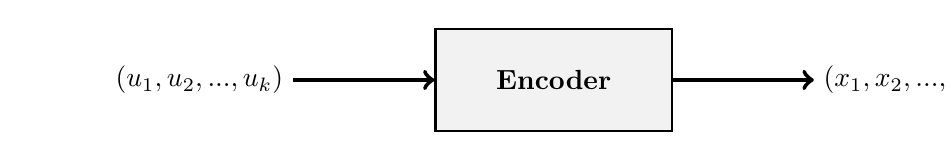
\begin{tikzpicture}
  \hspace{1cm}
  \node [] (u) {\((u_1,u_2,...,u_k\))};
  \node[
  right of=u,
  rectangle,
  draw,
  thick,
  fill=gray!10,
  minimum width=30mm,
  minimum height=13mm,
  xshift=35mm] (e) {\bfseries Encoder};

  \node[right of=e, xshift=35mm] (x) {\((x_1,x_2,...,x_n)\)};

  \draw[->,ultra thick] (u)--(e);
  \draw[->,ultra thick] (e)--(x);
\end{tikzpicture}

\vspace{4mm}
\noindent
Mathematically, the encoded vector \(x\) is obtained form the original vector \(u\) using the generator matrix \(G\) by the relation \(x=uG\) \cite{coding}.\\[5mm] To continue and complete the diagram.\\

\vspace{4mm}
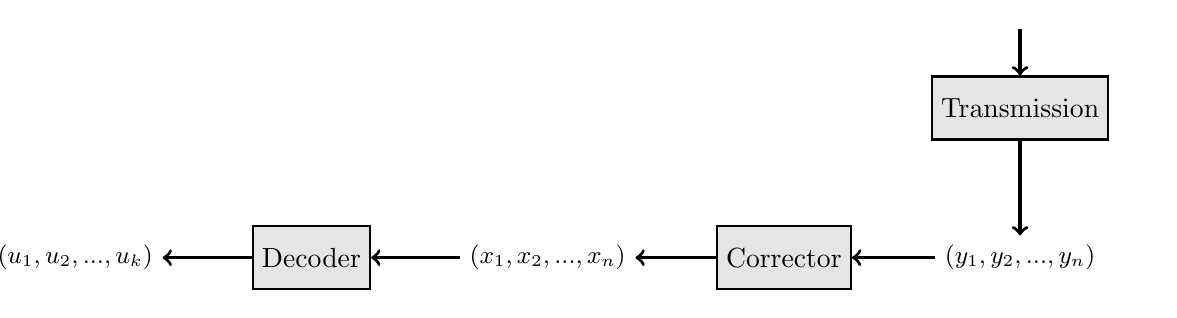
\begin{tikzpicture}
  \hspace{-5mm}
  \node[
  rectangle,
  draw,
  thick,
  fill=gray!20,
  minimum width=13mm,
  minimum height=8mm,
  ] (t) {Transmission};

  \node[below of=t, yshift=-9mm] (y) {\small \((y_1,y_2,...,y_n\))};

  \node[
  left of=y,
  rectangle,
  draw,
  thick,
  fill=gray!20,
  minimum width=13mm,
  minimum height=8mm,
  xshift=-20mm] (c) {Corrector};

  \node[left of=c, xshift=-20mm] (x) {\small \((x_1,x_2,...,x_n)\)};

  \node[
  left of=x,
  rectangle,
  draw,
  thick,
  fill=gray!20,
  minimum width=13mm,
  minimum height=8mm,
  xshift=-20mm] (d) {Decoder};

  \node[left of=d, xshift=-20mm] (u) {\small \((u_1,u_2,...,u_k\))};


  \draw[->,very thick] (0,1)--(t);
  \draw[->,very thick] (t)--(y);
  \draw[->,very thick] (y)--(c);
  \draw[->,very thick] (c)--(x);
  \draw[->,very thick] (x)--(d);
  \draw[->,very thick] (d)--(u);
\end{tikzpicture}

\vspace{9mm}
\section{Syndrome Decoding}
\begin{definition} \cite{error_correct}
  The syndrome of a vector \(y \in V\) is defined as \\ \(syn(y)=\begin{pmatrix}
    y.h_1\\
    y.h_2\\
    .\\
    .\\
    .\\
    y.h_{n-k}
  \end{pmatrix}\), \hspace{12mm} where \(\begin{pmatrix}
    h_1 \\ h_2\\ .\\ .\\ .\\ h_{n-k}
  \end{pmatrix}\) is the parity check matrix of \(C\).
\end{definition}
\vspace{3mm}
Now the code \(C\) is a subgroup of \(V\) under addition. Moreover, it is a normal subgroup of \(V\).
\begin{theorem} \cite{error_correct}
  Two vectors in \(V\) have the same syndrome if and only if they are in the same co-set of \(C\).
\end{theorem}
\clearpage

\subsection{Decoding Process}
Suppose the signal received is the vector \(y\).
\begin{enumerate}
\item First we determine its syndrome, \(syn(y)\).
\item Determine the co-set of \(C\) containing \(syn(y)\), say \(e + C\).
\item Then \(y=e+x\) for some \(x \in C\). This implies \(x=y-e\). Since \(x \in C\), this \(x\) is the required decoding of \(y\) \cite{error_correct}.
\end{enumerate}
This \(e\) is also called "error vector" \cite{error_correct}.
\vspace{2mm}

\begin{example}
  Consider a generator matrix \(G=\begin{pmatrix}
    1 & 0 & 1 & 0\\
    0 & 1 & 1 & 1
  \end{pmatrix}\). Then the parity check matrix is \(H=\begin{pmatrix}
    1 & 1 & 1 & 0\\
    0 & 1 & 0 & 1
  \end{pmatrix}\). And the code generated by \(G\) is  \(C=\{(0,0,0,0),(1,0,1,0),(0,1,1,1),(1,0,1,1)\} \;\; \subset GF(2^{4})\).\\

  Suppose the received vector is \(y=(1,1,1,0)\). Then \(y \not \in C\) so the information is distorted from the original information. To get the original information:\\
  \(syn(y)= \begin{pmatrix}
    y.h_1 \\ y.h_2
  \end{pmatrix} = \begin{pmatrix}
    1 \\ 1
  \end{pmatrix}\) where \(h_1\) is the first row and \(h_2\) is the second row of \(H\).\\
  Now if \(e=(0,1,0,0)\) then \(e+C=\begin{pmatrix}
    1 \\ 1
  \end{pmatrix}\) so \(y-e=(1,1,1,0)-(0,1,0,0)=(1,0,1,0) \in C\) is the original information \cite{error_correct}.

\end{example}


\section{Perfect Code}
The code \(C \subseteq V\) as of above is perfect if the union of all the spheres of radius \(t\) about its code-words is the vector space \(V\).\\
This code is \(C\) is called perfect because every received vector with the number of errors given by \(t\) can be decoded to a code-word of \(C\) \cite{error_correct}.

\begin{example}
  The code \(C=V\) is a perfect code. This code cannot correct any errors because every possible code word is in the \(C\). Therefore this perfect code is trivial \cite{error_correct}.
\end{example}

\begin{example}
  The general binary Hamming code \(H_r\), \(r \in \mathbb{N}\) whose parity check matrix \(H\) column consisting of non-zero r-tuples \cite{error_correct}.
\end{example}

\section{Cyclic Code}
The code \(C\) as of above is cyclic if \((a_0,a_1,...,a_{n-1}) \in C \implies (a_{n-1},a_0,...,a_{n-2}) \in C\).\\

Suppose \(C\) is a code over a Galois field \(F=GF(q)\). Then there exist a correspondence \(\Phi : C \mapsto F[x]/(x^n-1)\) such that \(\{(a_0,a_1,...,a_{n-1}),(a_1,...,a_{n-1},a_0),....,(a_{n-1},a_0,....,a_{n-2})\} \longmapsto a_0+a_1x+a_2x^2+...+a_{n-1}x^{n-1}\). \\

This map \(\Phi\) is homomorphism. This shows that the cyclic code \(C\) can be embedded into the ring \(R_n=F[x]/(x^n-1)\) \cite{error_correct}.
\vspace{5mm}
\begin{theorem} \cite{error_correct}
  \begin{enumerate}
  \item A subset \(S\) of \(R_n\) corresponds to a cyclic code if and only if \(S\) is an ideal of \(R_n\) and
  \item if \(S=(g(x))\) if and only if  \(g(x)\) divides \(x^n-1\).
  \end{enumerate}
\end{theorem}

\begin{tcolorbox}
  This theorem determines all cyclic codes. They are ideals of \(R_n\) and these ideals are generated by the polynomials that divides \(x^n-1\). Thus cyclic code have a generator polynomial which is computationally simpler than having a generator matrix. \\[2mm]
  This is where usages of polynomial representation of finite fields come into play and this is where cyclic code has advantage over general linear code.
\end{tcolorbox}

\vspace{5mm}
\begin{example}
  The divisors of \(x^3-1 \in F=GF(2^{3})\) are \(1, x+1, x^2+x+1, x^3-1\).\\
  For \(g(x)=x+1\) we have \(F[x]/(g(x))=\{(0),(1+x),(1+x^2),(x+x^2)\}\) so the corresponding cyclic code is \(\{(0,0,0),(1,1,0),(1,0,1),(0,1,1)\}\) \cite{error_correct}.
\end{example}

\vspace{7mm}
``Similar to general linear codes which are defined using the generator matrix or the parity-check matrix, cyclic codes are defined using generator polynomial or parity-check polynomial and the advantage of cyclic code is that there exists efficient algebraic decoding algorithm for them'' \cite{coding}.

\clearpage
\subsection{Usages}
\begin{enumerate}
\item The \((3,1)\) binary code is used in the short-range wireless communication system like \(Bluetooth^{TM}\) \cite{wireless}.
\item The Hamming Code \((7,4)\) is used in memory devices like RAM \cite{coding}.

  \item The Cyclic codes are used in storing data in CDs and DVDs \cite{coding}.
  \end{enumerate}
  \vspace{9mm}

  \begin{figure}[h]
    \centering
    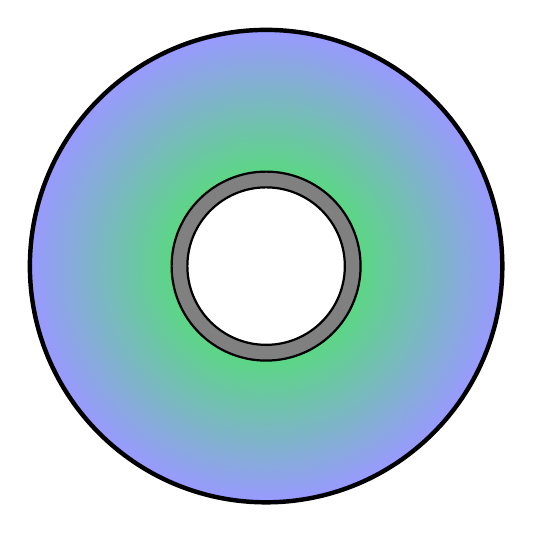
\begin{tikzpicture}
      \draw [ultra thick, outer color=blue!40, inner color= green!80] (0,0) circle [radius=3];
      \draw[thick, fill=gray] (0,0) circle [radius=1.2];
      \draw[thick, fill=white] (0,0) circle [radius=1];
    \end{tikzpicture}
    \caption{\footnotesize A CD}
    \end{figure}

\chapter{Application in Cryptography}
\section{Cryptography}
It is the science of safe-guarding information by converting the original message into something unreadable.\\
Galois Fields are the life of modern cryptography used in digital communication.

\section{Advance Encryption Standard(AES)}
The Advance Encryption Standard is a Computer Security Standard for cryptography which is approved by the ``Federal Information Processing Standards Publications'' of USA which became effective on May 26, 2002. ``The AES algorithm is a \textit{symmetric block cipher} that can encrypt and decrypt digital information'' \cite{aes}. Symmetric key cryptography is used to share information between two parties where the two parties share a secret ``key'' and a public encryption algorithm.\\

``In 2000, National Institute of Standards and Technology(NIST) announced the selection of the ``Rijndael'' block cipher family as the winner of the AES competition and since then AES has been the standard for digital cryptography'' \cite{aes}. ``The Rijendael block cipher was developed by two Belgian cryptographers, \underline{Vincent Rijmen and Joan Daemen}'' \cite{aes}.\\

The generic algorithm of AES consists of smaller sub-algorithms namely\\ ``Sub-Bytes, Shift-Rows, Mix-Columns and Add-Round-Key'' \cite{aes}.

\begin{table}[h!]
  \centering
\begin{tabular}{|l|l|}
  \hline
  Bit & \hspace{7mm}''A binary digit: 0 or 1'' \cite{aes}.\\
    \hline
  Byte & \hspace{7mm}''A sequence of 8 bits'' \cite{aes}.\\
    \hline
  Block & \hspace{7mm}''A sequence of bits of a fixed length'' \cite{aes}.\\
  \ & \hspace{13mm}''In this Standard, block consists of 128 bits'' \cite{aes}.\\
    \hline
  Block cipher &  \hspace{7mm}''A family of permutations of blocks'' \cite{aes}.\\
    \hline
  Key & \hspace{7mm}''The parameter that selects the permutation'' \cite{aes} \\
  \ & \hspace{13mm}from the block cipher.\\
    \hline
\end{tabular}
\caption{\small Terms and their meanings.}
\end{table}


\vspace{7mm}
\section{The Cipher(Algorithm)}
\subsection{The State}
First the data is broken into blocks and each block is broken into smaller chunks of a size byte (16 bytes for a block of size 128 bits). This block is then represented in a  which consisting of bytes of the word. This matrix is called the State.\\
Mathematical operations are not applicable to the data directly so the significance of this step is to make the data applicable for mathematical operations.\\
For the 128-bit key encryption the algorithm forms a \(4 \times 4\) matrix with each entry of a size one byte. This matrix can afford to evaluate a data of size 16 byte at a time \cite{aes}.

\vspace{3mm}
\subsection{Sub-Bytes}
In this step, first each byte of the matrix is replaced with its multiplicative inverse if it has one. Then it transforms each bytes using an invertible affine transformation, \(x \mapsto Ax+b\) \cite{aes}.

\subsection{ Mathematical Preliminaries}
Each byte in the state i.e each entry in the matrix, is interpreted as one of the 256 elements of a finite field \(GF(2^8)\). Then the addition, multiplication operations are performed according to the respective field operations of the field \(GF(2^8)\).

\vspace{3mm}
\subsection{Shift-Rows}
In this step entries of a row is shifted to scramble data. Row-n shifted to the left by \(n-1\) unit. Here,\\
\(1-1=0\), so row-1 is left unchanged. \(2-1=1\), so row-2 is shifted to the left by 1 unit and row-3 by 2 unit and so on as shown below \cite{aes}.

\vspace{3mm}
If \(A=\begin{bmatrix}
    a_{11}&a_{12}&a_{13}&a_{14}\\
    a_{21}&a_{22}&a_{23}&a_{24}\\
    a_{31}&a_{32}&a_{33}&a_{34}\\
    a_{41}&a_{42}&a_{43}&a_{44}
    \end{bmatrix}\) \hspace{3mm} then \(A'=\begin{bmatrix}
    a_{11}&a_{12}&a_{13}&a_{14}\\
    a_{22}&a_{23}&a_{24}&a_{21}\\
    a_{33}&a_{34}&a_{31}&a_{32}\\
    a_{44}&a_{41}&a_{42}&a_{43}
    \end{bmatrix}\) \vspace{2mm} \\[3mm] is the matrix after Shit-Row

\subsection{Mix-Columns}
In this step each column is transformed using a linear transformation, \(c \mapsto Bc\) where \(c\) is a column of the matrix obtained above. Since linear transformation is invertible this step is invertible. Note every step of this algorithm must be invertible to be able to decrypt the data \cite{aes}.

\subsection{Add-Round-Key}
This is the step where the encrypted data gets uniqueness. Each user is assigned an "unique key" and this key is added to the matrix obtained from the last step \cite{aes}.

\subsection{Algorithms}
\begin{tcolorbox}[colback=gray!20, colframe=blue!30, left=2cm, title={\small \bfseries \textcolor{black}{Encryption Algorithm}}, width=15cm]
\begin{verbatim}
procedure CIPHER(state, key)
    for round from 1 to 9 do
        1)   SUBBYTES(state)
        2)   SHIFTROWS(state)
        3)   MIXCOLUMNS(state)
        4)   ADDROUNDKEY(state, key)
    end for
end procedure
\end{verbatim} \cite{aes}
\end{tcolorbox}

\vspace{7mm}
\begin{tcolorbox}[colback=gray!20, colframe=blue!30, left =2cm, title={\small \bfseries \textcolor{black}{Decryption Algorithm}}, width=15cm]
\begin{verbatim}
procedure CIPHER(state, key)
    for round from 1 to 9 do
        1)   InvADDROUNDKEY(state, key)
        2)   InvMIXCOLUMNS(state)
        3)   InvSHIFTROWS(state)
        4)   InvSUBBYTES(state)
    end for
end procedure
\end{verbatim}\cite{aes}
\end{tcolorbox}

\section{Illustration}
Let us encrypt the sentence "Fun Cryptography". This consists of exactly 16 characters.\vspace{2mm}

\begin{enumerate}
\item First we write the ASCII representation of each character of the sentence as shown below. We do so because the ASCII representation gives the binary representation of each character which has a size of a byte. The ASCII representation of "F" is \(70\) which is \(01000110\) in binary.\vspace{2mm}

  \[\begin{bmatrix}
      70 & 117 & 110 & 32 \\
      67 & 114 & 121 & 112\\
      116 & 111 & 103 & 114 \\
      97 & 112 & 104 & 121
    \end{bmatrix}=
    \begin{bmatrix}
      01000110 & 01110110 & 01101110 & 00010000 \\
      01000011 & 01110010 & 01111001 & 01110000\\
      01110100 & 01101111 & 01100111 & 01110010 \\
      01100001 & 01110000 & 01101000 & 01111001
    \end{bmatrix}
  \]

  \vspace{5mm}

\item After performing Sub-Bytes, Shift-Rows, Mix-Columns, we get the following matrix. \vspace{2mm}

  \[\begin{bmatrix}
      11100111 & 00011000 & 00100100 & 01110000\\
      00101010 & 10101011 & 00111001 & 01100011\\
      00010101 & 01100101 & 11110111 & 10100111\\
      10101011 & 11110110 & 00000011 & 10100100
    \end{bmatrix}=
    \begin{bmatrix}
      231 & 24 & 36 & 112\\
      42 & 171 & 57 & 99\\
      21 & 101 & 247 & 167\\
      171 & 246 & 3 & 164
    \end{bmatrix}
  \]
  \vspace{5mm}

\item We have omitted the Add-Round-Key step just for the sake of simplicity. The matrix obtained at last in step-2 translates to something different from our original sentence.

  \vspace{5mm}

\item The decryption process is applying the inverse of the encryption process \cite{aes}.
\end{enumerate}


\backmatter
\chapter*{Conclusion}
\addcontentsline{toc}{chapter}{\bfseries Conclusions}
\chapter*{Conclusions}
The Galois theory that begun in the 19th century due to the french mathematician \textit{Évariste Galois} is still a relevant field of research today. Over the 200 years this theory has found its development as a linking theory of the two main theories: Group Theory and Field theory. It has found its applications in both pure and applied mathematics; where-ever ``Field Theory'' has anything to do with.\\[3mm]
Many concepts of Abstract algebra, Algebraic number theory, Algebraic geometry, etc rely heavily on Galois theory because they are developed on field extensions, and the computer science relies heavily on Galois field.


\bibliographystyle{plain}
\bibliography{bib_database/myref}

\end{document}


%%% Local Variables:
%%% mode: latex
%%% TeX-master: t
%%% End:
